% !TEX root = ../Poissons.tex

\section{Facets of the diagonal} 
\label{s:facets}

In this section we establish a bijection between the facets of $\triangle$ and a family of pairs of unordered partitions introduced and enumerated in a series of 3 papers \cite{chen1969computer,chen1971tables,kajitani1982number}. An intermediary bijection to a type of bipartite tree is of particular importance and provides [...].
In particular, we obtain that the number of facets in the image of the diagonal $\triangle_n$ of the $n$-dimensional permutahedron is $2(n+1)^{n-2}$ (\OEIS{A007334}), and more precisely that the pairs of dimensions $(k,n-k)$ are counted by the formula $\frac{1}{k+1}\binom{n+1}{k}(k+1)^{n-k}(n+1-k)^{k}$. 
\Guillaume{OEIS ref?}


\subsection{Essential complementary partitions and bipartite trees}
Let us recall some basic definitions and results from the series of papers \cite{chen1969computer,chen1971tables,kajitani1982number}.

\begin{definition}
A set of \emph{distinct representatives} of a partition $\sigma_I$ is a set $R\subset [n]$ such that $\forall i \in I,|\sigma_i \cap R| = 1$.
\end{definition}

\begin{definition}
A pair of partitions $(\sigma_I,\tau_J)$ is said to be \emph{complementary} if there exists $R\subset [n]$ and $r \in R$ such that $R$ and $([n]\setminus R) \cup \{r\}$ are distinct representatives of $\sigma_I$ and $\tau_J$, respectively.
It is furthermore \emph{essential} if there does not exist proper subsets $ I'\subset I$, $J'\subset J$ and $K \subset [n]$ such that $(\sigma_{I'},\tau_{J'})$ is a complementary partition of $K$.
\end{definition}

We shall denote the set of all essential complementary pairs of partitions by $\EC$.
Let us emphasize that the pairs of partitions of $\EC$ are \emph{unordered}.

\Guillaume{Notations to be uniformized from here}

\begin{example}
n=2, n=3
\end{example}
\Kurt{To do}

A \emph{tree} is a simply connected graph with no cycles. 
A \emph{bipartite graph} is a graph whose vertices are partitioned into two sets such that vertices in one set are only adjacent to vertices in the other, we say it is \emph{ordered} if one of the sets is considered smaller than the other and we denote the partition $(V_L,V_R)$. 
We say a graph with $n$ edges is \emph{edge labelled} if there exists a bijection between the edges and $\{1,\dots,n\}$.
Let $\BT$ denote the set of edge labelled ordered bipartite trees.

\begin{proposition} [{\cite[Theorem 3]{kajitani1982number}}] 
\label{EC Graph Bijection}
Essential complementary partitions and labelled bipartite trees are in bijection through $G:\EC \to \BT$ and $P:\BT \to \EC$, where
\begin{itemize}
    \item $G$ takes a pair $(P_L,P_R)$ and constructs partitioned vertices $(V_L,V_R)$. For each $i \in  \{1,\dots,n\}$ an edge is added between $v_l$ and $v_r$ if $i\in P_l$ and $i \in P_r$. 
    \item $P$ takes a tree from $\BT$ and labels the vertices $(V_L,V_R)$ by the edges which are adjacent to them. The labels of the vertices can then be interpreted as a pair of partitions.
\end{itemize}
\end{proposition}
\Guillaume{Consider changing notation for functions vs sets}

\begin{figure}
\begin{center}
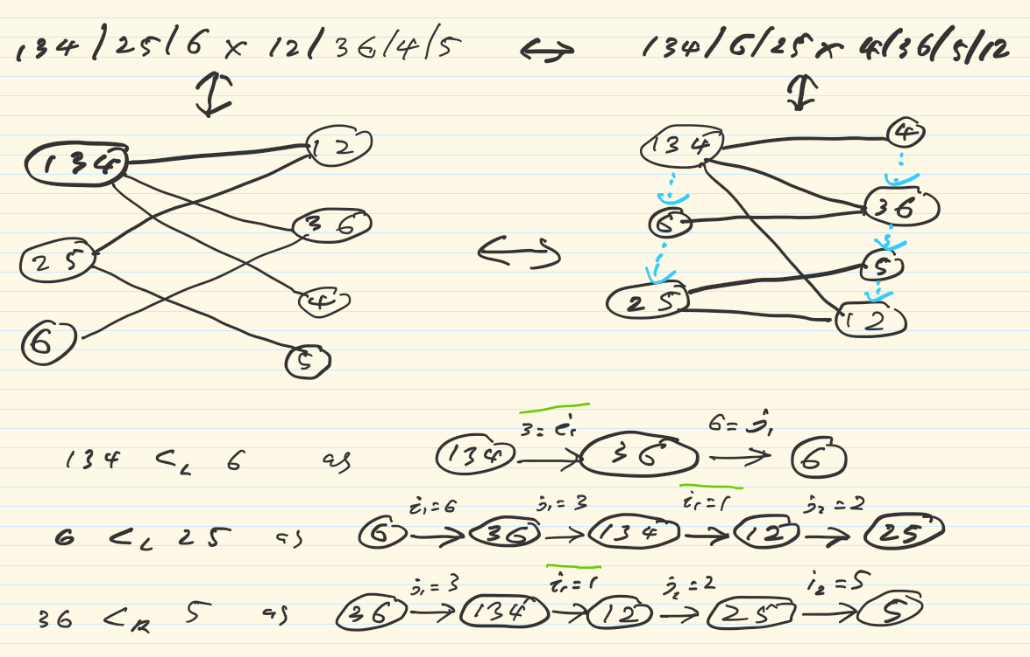
\includegraphics{Images/bijections_example.png}
\end{center}
\caption{The bijection between ordered partitions and bipartite trees.}
\end{figure}

\begin{corollary}[\cite{kajitani1982number}]
The number of essential complementary partitions is $|\EC_n| = 2(n+1)^{n-2}$.
\end{corollary}

\subsection{Bijection with the facets of the diagonal}

In this section we denote by $\OP$ be the set of pairs of ordered partitions of $[n]$ labeling \emph{facets} of the diagonal $\triangle$.

\begin{thm}
\label{thm:facets}
Facets of the diagonal and essential complementary partitions are in bijection through the inverse functions $u:\OP \to \EC$ and $o:\EC\to \OP$, where
\begin{enumerate}
    \item The function $u$ forgets the order of the ordered partition pair.
    \item The function $o$ uniquely orders an essential complementary partition pair via the minimal $(I,J)$-pairs defining the diagonal. 
\end{enumerate}
\end{thm}
We shall prove this theorem by establishing the necessary total order, showing that the functions are well defined, and then showing that they are injective.

\begin{lemma} 
\label{l:u-well-defined}
The function $u:\OP \to \EC$ that forgets the order in a pair of partitions is well defined.
\end{lemma}
\begin{proof}
Let $P \in \OP_n$. Then $G(u(P))$ is a graph with $l+r=n+1$ vertices, and $n$ edges. Furthermore, as no vertices can be isolated it must be the case that this graph is a tree. 
It is straightforward to verify that $G(u(P))$ must be labeled bipartite tree, but here is how we may explicitly produce the necessary distinct representatives using an algorithm of \cite[Theorem 2]{kajitani1982number}.

Let $G'$ be a copy of $G(u(P))$. 
While there is a vertex of degree $1$ in $G'$ delete it and add the sole edge of that vertex as a distinct representative of the corresponding partition of that vertex. 
As $G'$ is a tree this process can continue until there is a single edge connecting two vertices of degree $1$. 
This edge specifies the element $p$ of the distinct representatives.
\end{proof}

\begin{construction} 
\label{Order Lemma}
For $P=(P_L,P_R) \in \EC$ an essential complementary pair, we construct total orders on $P_L$ and $P_R$ in three steps:
\begin{enumerate}
    \item For $l,l' \in L$ there exists a unique minimal set of edges $p_{l,l'}$ of even cardinality connecting $V(P_l)$ and $V(P_{l'})$ in $G(P)$ (similar for $R$). We partition this set of edges as $I\cup J$ where $I$ and $J$ are each pairwise non-adjacent, and $I$ contains the minimal edge.
    \item Orient each path so that $I$ points left to right, and $J$ points right to left (same orientation for $P_L$ and $P_R$). 
    \item We say $P_l< P_{l'}$ (or $P_r < P_{r'}$) if the constructed path points from $V(P_l) \to V(P_{l'})$ ($V(P_r) \to V(P_{r'})$.
\end{enumerate}
\end{construction}

\begin{proof}
We first show our binary relation is well defined before verifying that it defines a total order on $G(P)$ and hence $P$ via the bijection of \cref{EC Graph Bijection}.

As $G(P)$ is a bipartite tree, every vertex is connected, and every path connecting two vertices on the same side must be of even length. 
As $I$ and $J$ are each pairwise non-adjacent, they must partition the path in an alternating fashion i.e. $p=(I_{i_1},J_{j_1},I_{i_2},J_{j_2},..., )$, hence we can orient the path by forcing $I$ to point left and $J$ to point right.

This order is clearly total, reflexive (by convention) and anti-symmetric, what remains to be checked is its transitivity. 

Let $p_{ab}$ denote the unique maximal path between two vertices $a$ and $b$ on the left of $G(P)$, that is two blocks of $P_L$. 
Let $I_{ab}$ denote the set of left-to-right edges in this path, and let $J_{ab}$ denote its complement. 
Then, we have 
\begin{equation}
    \label{eq:order}
    a < b \iff \min(I_{ab}\cup J_{ab})=\min(I_{ab}) \ . 
\end{equation}
Suppose now that $a < b$ and $b < c$.
Since $p_{ac}= (p_{ab} \cup p_{bc}) \setminus (p_{ab} \cap p_{bc})$, we have $$ I_{ac}=(I_{ab}\cup I_{bc}) \setminus (J_{ab} \cup J_{bc}) \text{ and } J_{ac}=(J_{ab}\cup J_{bc}) \setminus (I_{ab} \cup I_{bc}) \ , $$ and from the condition (\ref{eq:order}) above it is clear that $\min(I_{ac}\cup J_{ac})=\min(I_{ac})$, which completes the proof of the transitivity for the total order on $P_L$. 
The proof for $P_R$ is similar. 
\end{proof}

This order far from being arbitrary provides the unique way to order an essential complementary partition pair into an ordered partition pair of $\triangle$, as we shall demonstrate next.

First we need a geometrical lemma. 
\begin{proposition}
    The paths between adjacents vertices of $P_L$ or $P_R$ are in bijection with the minimal $(I,J)$-pairs.
\end{proposition}

\begin{proof}
    By \cref{p:minimal-IJ-pairs}, it suffices to show that the paths between adjacent vertices of $P_L$ are in bijection with the solutions of the system of equations of the form $(\rho^1,\sigma^2)$. 
    To ease notation let us write $\rho$ for $\rho^1$ and $\sigma$ for $\sigma^1$. 
    Suppose that $\rho$ is obtained from $\sigma$ by merging the two blocks $\sigma_a$ and $\sigma_b$. 
    The two equations $\langle \vec \sigma_a, x \rangle =0$ and $\langle \vec \sigma_b, x \rangle =0$ now become $\langle \vec \sigma_a + \vec \sigma_b, x \rangle =0$; nothing else changes in the system. 
    Since the solution to the system $(\sigma^1,\sigma^2)$ was $x=0$, now the solution is of dimension $1$, and it is given precisely by the path between $a$ and $b$ in $G(P)$.
    Such a path is given by an alternating sequence of vertices and edges $\sigma_1:=\sigma_a, e_1, \sigma_2, e_2, \ldots, e_{k-1}, \sigma_k:=\sigma_b$. 
    Every edge $e_i \in \{1,\ldots, n\}$ is by definition the intersection $\sigma_{i} \cap \sigma_{i+1}$; thus it is the only common non-zero coordinate between $\vec \sigma_{i}$ and $\vec \sigma_{i+1}$.
    Thus the path encodes the series of equations $x_{e_1}+x_{e_{k-1}}=0$, $x_{e_1}+x_{e_2}=0$, $x_{e_2}+x_{e_3}=0$, $\ldots$, $x_{e_{k-2}}+x_{e_{k-1}}=0$. 
    Thus, $x_{e_1}=1$, $x_{e_2}=-1$, $x_{e_3}=1$, $\ldots$, $x_{e_{k-2}}=1$, $x_{e_{k-1}}=-1$ is a basis of one-dimensional space of solutions, and it gives the corresponding minimal $(I,J)$-pair. 
\end{proof}

\begin{lemma} 
\label{o well defined}
The function $o:\EC \to \OP$ that orders an essential complementary pair is well defined.
\end{lemma}

\begin{proof}
Let $P=(P_L,P_R) \in \EC$ and consider $o(P)$. 
We first show that every $(I,J)$-condition, for $(I,J) \in D(n)$, which corresponds to a path between vertices is satisfied. 
In particular, this statement will be true for minimal $(I,J)$-pairs, which will be enough in virtue of \cref{p:minimal}. 
Suppose $I,J$ corresponds to a path between two vertices on the left, i.e.
\begin{align*}
    V(P_l) = V_{L_1} \xrightarrow{i_1} V_{R_1}\xrightarrow{j_1} V_{L_2} \xrightarrow{i_2}... \xrightarrow{i_{k}} V_{R_{k-1}} \xrightarrow{j_k} V_{L_k}=V(P_{l'})
\end{align*}
By construction we have that $I = \{i_1,...,i_k\},J=\{j_1,...,j_k\} \in D(n)$ (note we are ordering $I$ and $J$ by the path, so it is not necessarily the case that $\min I = i_1$). 
Furthermore, each sub partition of $P_R$ either contains a single element of $I$ and a single element of $J$, or it contains no elements of $I$ and no elements of $J$. 
As such for any ordering of the sub-partitions of $P_R$ we have that 
\begin{align*}
    \forall m, \bigg|\bigcup_{1\leq k \leq m} P_{R,k} \cap I \bigg| = \bigg|\bigcup_{1\leq k \leq m} P_{R,k} \cap J \bigg|
\end{align*}
Hence in order for this $D(n)$ condition to be satisfied it must be the case that for some ordering of the sub-partitions of $P_L$ we have
\begin{align*}
    \exists m, \bigg| \bigcup_{1\leq k \leq m} P_{L,k} \cap I \bigg| > \bigg|\bigcup_{1\leq k \leq m} P_{L,k} \cap J \bigg|
\end{align*}
Every sub-partition of $P_L$ excluding the $l$th and $l'$th either contains no elements of both $I$ and $J$, or it contains a single element of $I$ and a single element of $J$. 
So the only way for the condition to be satisfied is for $P_l$ to come before $P_{l'}$, which is precisely what is required by the total order.

If $I,J$ correspond to a path between two vertices on the right,
\begin{align*}
    V(P_r) = V_{R_1} \xrightarrow{j_1} V_{L_1}\xrightarrow{i_1} V_{L_2} \xrightarrow{j_2}... \xrightarrow{j_{k}} V_{L_{k-1}} \xrightarrow{1_k} V_{R_k}=V(P_{r'})
\end{align*}
then a similar chain of logic implies we must have an ordering of the sub-partitions of $P_R$ such that
\begin{align*}
    \exists m, |\bigcup_{1\leq k \leq m} P_{R,k} \cap I| < |\bigcup_{1\leq k \leq m} P_{R,k} \cap J|
\end{align*}
and this can only happen if $P_r$ comes before $P_{r'}$.
\end{proof}

\begin{rem}
    It would be interesting to know if there is a geometrical interpretation of the paths that are not between adjacent vertices. 
\end{rem}

To complete the proof of \cref{thm:facets}, it remains to show that both $u:\OP \to \EC$ and $o:\EC\to \OP$ are injective, with the other function being their inverse.

\begin{proof}[{Proof of \cref{thm:facets}}]
The forgetful function $u$ is clearly the inverse to $o$ as forgetting any assigned order will clearly return the original essential complementary partition pair. 
The ordering function $o$ is the inverse to $u$ as it returns the sole ordering of the sub-partitions which is compatible with the $D(n)$ conditions.
\end{proof}

\subsection{Combinatorial formula for facets of the diagonal}

From \cref{thm:facets}, we can deduce a formula for the number of facets of the diagonal:

\begin{proposition}
The number of pairs of ordered partitions of dimension $(k,n-k)$ which correspond to facets of the diagonal is given by: 
\begin{equation}
\frac{1}{k+1}\binom{n+1}{k}(k+1)^{n-k}(n+1-k)^{k}.
\end{equation}
\end{proposition}

\begin{proof}
According to Theorem \cref{thm:facets}, pairs of ordered partitions of dimension $(k,n-k)$ which correspond to facets of the diagonal are in one-to-one correspondence with bipartite trees with $k+1$ black vertices, $n-k+1$ white vertices and $n+1$ edges labeled from $1$ to $n+1$.

We do not prove exactly here the proposition but a slightly modified version: 
Rooted bipartite trees with $k+1$ black vertices and $n-k+1$ white vertices such that:
\begin{itemize}
\item a black vertex is distinguished and called \emph{the root}
\item the $n+1$ non-root vertices are labeled,
\item every label between $1$ and $n+1$ is used exactly once.
\end{itemize}
are counted by:
\begin{equation}
\binom{n+1}{k}(k+1)^{n-k}(n+1-k)^{k}.
\end{equation}

Let us construct such a bipartite tree. 

First, there are $\binom{n+1}{k}$ ways to  choose the labels for black vertices (white vertices being labeled by the non-chosen labels). 
We denote by $\mathcal{B}$ this set of labels.

Moreover, the labeled black vertices are different from the root, hence they should have a white parent : there are $n+1-k$ ways to choose the parent of any labeled black vertex. 
We thus have  $(n+1-k)^{k}$ ways to build corollas with labeled black leaves and a white root, called bi-colored corollas (or sometimes just corollas) in the sequel.

Finally, we arrange bi-colored corollas in a rooted bipartite tree by adapting the algorithm which convert a Pr\"ufer code to a tree. 
Here what is called \emph{Pr\"ufer code} is a word of length $n-k$ over the alphabet $\mathcal{B} \cup \{\bullet\}$, where $\bullet$ stands for the non-labeled black vertex. 
Let us start with a word $c=c_1 \ldots c_{n-k} \bullet$ of length $n-k+1$ and the set $\mathcal{T}=\mathcal{S} \cup \{\bullet\}$ of $n-k+2$ bi-colored corollas augmented with the unlabeled black vertex. 
We apply Algorithm \ref{PruferWtoT}. Let us first prove it termination and correctness. The equality 
$\operatorname{length}(c)=\operatorname{Card}(\mathcal{T})-1$ is a loop invariant for the While loop: indeed at each iteration of the loop, the length of $c$ and the number of elements in $\mathcal{T}$ decrease exactly by one. It ensures the termination of the loop and the fact that $\mathcal{T}$ contains a unique element when exiting the loop. Moreover, the set of trees $\mathcal{T}$ contains at each steps exactly one unlabeled black vertex, $k$ labeled black vertices and $n-k+1$ white vertices. Finally, when adding an edge between two trees, one can only get a tree. Moreover, as the edge is added between a white root and the label of a black vertex, the obtained tree is indeed bipartite.

\begin{algorithm}[!ht]
\DontPrintSemicolon
  
  \KwInput{a word $c=c_1 \ldots c_{i}$ and a set $\mathcal{T}$ of $i$ bi-colored trees with white root and one bi-colored tree with an unlabeled black root}
  \KwOutput{a bipartite rooted tree}
  \While{$\operatorname{length}(c)>0$}{
      \tcc{loop invariant: $\operatorname{length}(c)=\operatorname{Card}(\mathcal{T})-1$, at each iteration, the length of $c$ decreases by $1$}
      t $\leftarrow \min\{a \in \mathcal{T} |$ none of the $c_i$ is a label in $a\}$ \tcp*{Here the order is given by the order on the labels of the root (as the tree with a black root does not satisfy the condition)}
      p $\leftarrow$ tree of $\mathcal{T}$ to which belongs the first letter of $c$ \tcp*{Note that it cannot be t itself}
      Remove t and p from $\mathcal{T}$ \tcp*{Decrease the cardinality of $\mathcal{T}$ by two}
      Add an edge between the root of $t$ and the first letter of $c$ and add the obtained tree to $\mathcal{T}$ \tcp*{Increase the cardinality of $\mathcal{T}$ by one}
      Remove the first letter of $c$ \tcp*{Decrease the length of $c$ by one}
  }
  {Return the unique element of $\mathcal{T}$}
  \caption{Pr\"ufer algorithm : from a word to a tree \label{PruferWtoT}}
\end{algorithm}

To prove that this algorithm defines a bijection between the pairs of Pr\"ufer code and set of bipartite rooted trees, let us give the algorithm which convert a rooted bipartite tree in such a pair in Algorithm \label{PruferTtoW}.


\begin{algorithm}[!ht]
\DontPrintSemicolon
  
  \KwInput{a bipartite rooted tree $A$}
  \KwOutput{a word $c=c_1 \ldots c_{i}$ and a set $\mathcal{T}$ of $i$ bi-colored trees with white root, except one bi-colored tree with an unlabeled black root}
  $c \leftarrow$ empty word \tcp*{}
  $\mathcal{T} \leftarrow$ empty set \tcp*{Initialization}
  \While{$A$ has more than one vertex}{
      \tcc{At each iteration, the number of white vertices decreases by $1$}
      t $\leftarrow \min\{w \in \mathcal{T} | w$ is a white vertex whose children are leaves $\}$ \tcp*{Here the order is the one on white labels}
      $c \leftarrow c$ concatenated with label of the parent of t \tcp*{This label is a black vertex}
      Remove the edge between t and its parent: the root part goes in $A$ and the corolla in $\mathcal{T}$ \tcp*{Increase the cardinality of $\mathcal{T}$ by one}}
  {  Return the pair $(c,\mathcal{T} \cup A)$}
  \caption{Pr\"ufer algorithm : from a tree to a word \label{PruferTtoW}}
\end{algorithm}

This second algorithm terminates as the number of white vertices decreases strictly by one at each iterations. Moreover, every letter added to $c$ is the label of a black vertices, and every tree added to $\mathcal{T}$ is a bi-colored corolla or $\bullet$ (the tree with only the non-labeled black root). Finally, the cardinality of the set of bipartite trees is one more than the length of $c$. As this algorithm is the classical reverse algorithm of the first one, it ends the proof.
\BDO{Do I need to add more details ?}
\end{proof}

\begin{example}
\begin{figure}[!h]
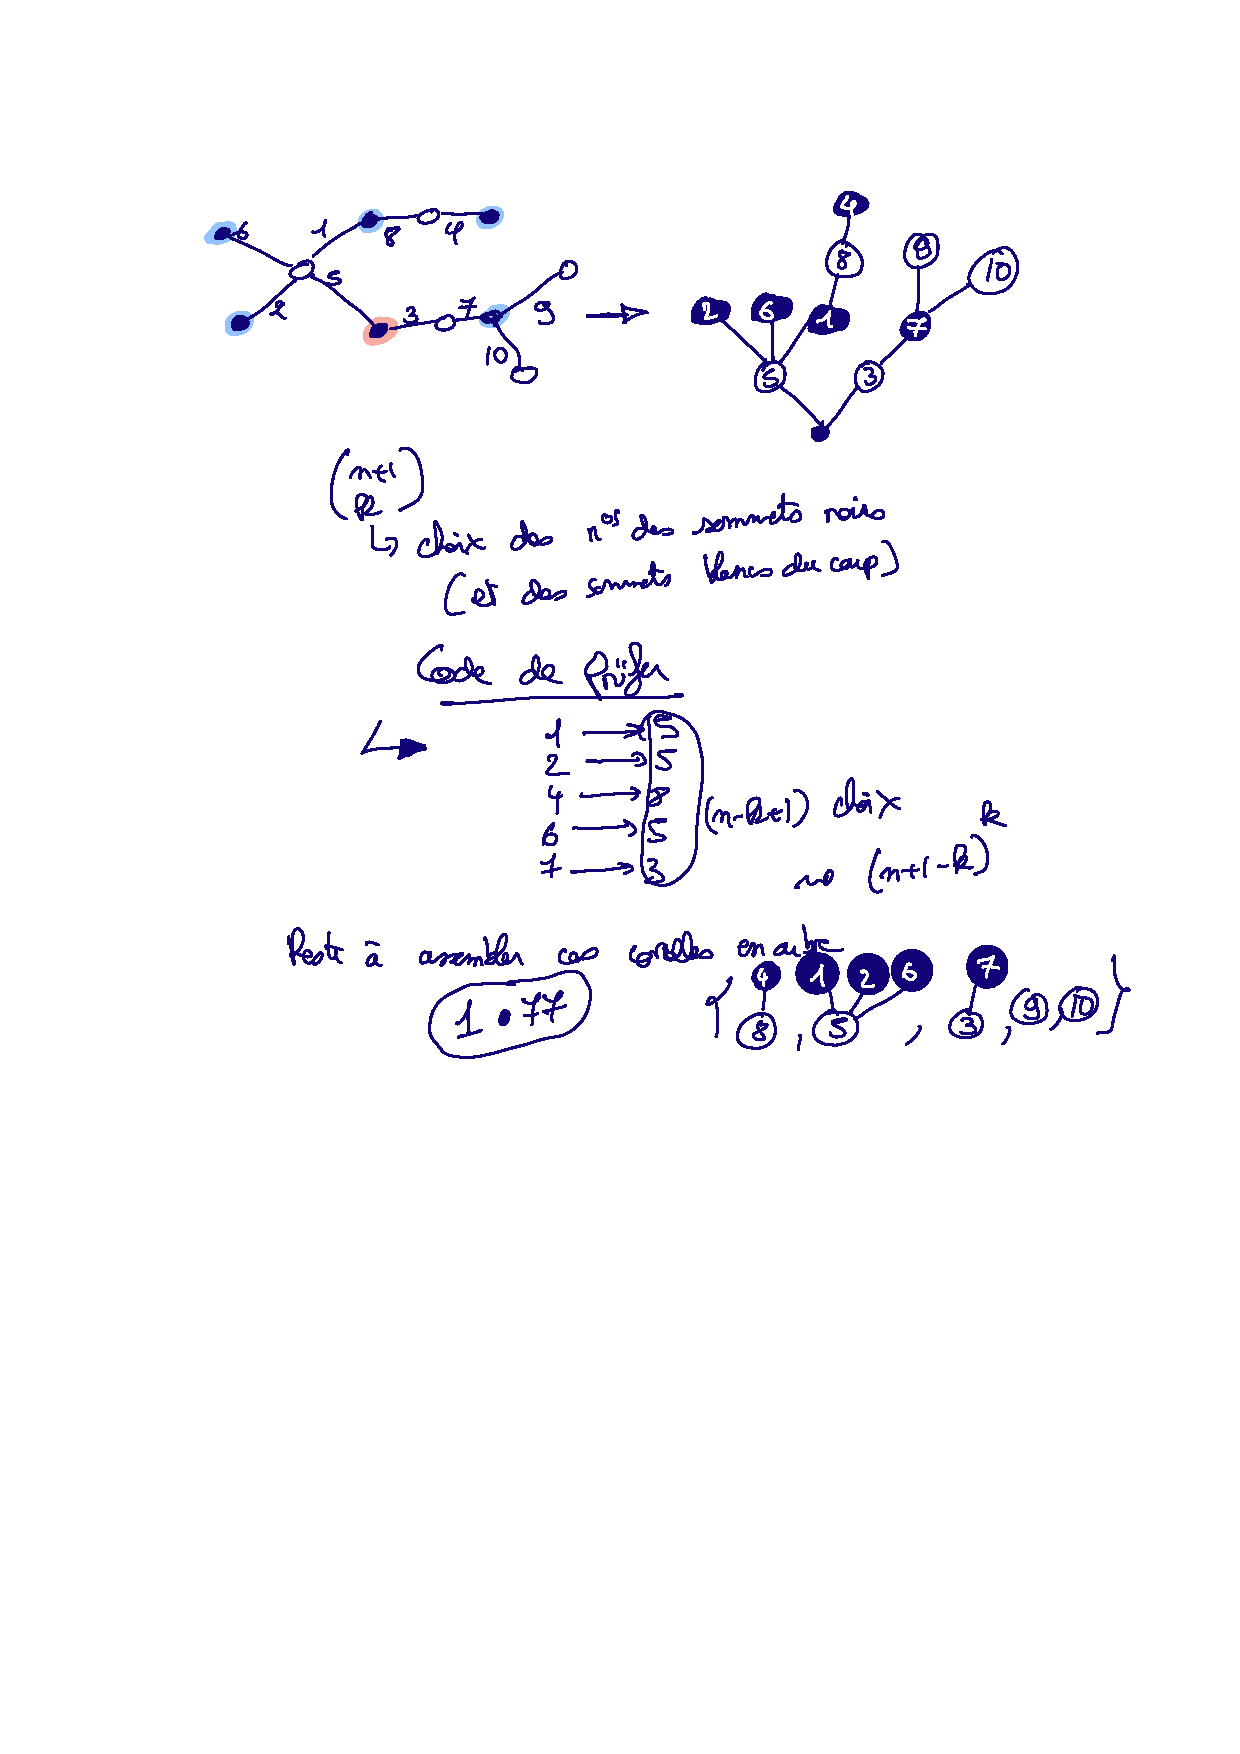
\includegraphics[scale=0.5]{Images/ExplePrufer.pdf}
\end{figure}
\BDO{Pr\"ufer algorithm applied on an example : TO DO}
\end{example}

\Guillaume{New section?}

\subsection{The Saneblidze--Umble description}

Here we prove that the diagonal $\OP$ admits a combinatorial description completely analogous to that of the Saneblidze--Umble diagonal \cite{SaneblidzeUmble04}. 
A direct corollary is that the two diagonals are in bijection, and moreover that the SU diagonal can be obtained from a certain choice of chambers in the fundamental hyperplane arrangements of the permutahedra, resolving a conjecture made in \cite{LA21}.
In particular, this provides an alternative proof that all known diagonals on the associahedra agree \cite{saneblidzeComparingDiagonalsAssociahedra2022}.

Given any permutation, one can canonically produce a facet of the diagonal in the following way. 

\begin{definition}
    A pair of ordered partitions $(\sigma,\tau)$ is called \emph{strong complementary} if $\sigma$ is obtained from a permutation by merging the adjacent elements which are descreasing, and $\tau$ is obtained from the same permutation by merging the adjacent elements which are increasing.
\end{definition}

An example is shown in \cref{fig:strong-complementary}.
The same argument as in \cref{l:u-well-defined} shows that the underlying pair of partitions is an essential complementary pair. 
Moreover we see directly that any path between adjacent vertices has length $2$, and that its minimum is always traversed from left to right, hence all strong complementary pairs are in $\OP$. 

\begin{figure}[h!]
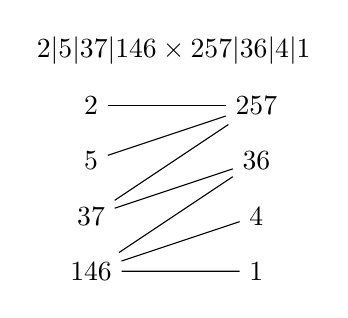
\begin{tikzpicture}[scale=.7]  
\node (p) at (0, 0) {$2|5|37|146 \times 257|36|4|1$};
\node (1) at (-1.5, -1) {$2$};
\node (2) at (-1.5, -2) {$5$};
\node (3) at (-1.5, -3) {$37$};
\node (4) at (-1.5, -4) {$146$};
%
\node (5) at (1.5, -1) {$257$};
\node (6) at (1.5, -2) {$36$};
\node (7) at (1.5, -3) {$4$};
\node (8) at (1.5, -4) {$1$};
%
\draw[-] (1)--(5); 
\draw[-] (2)--(5); 
\draw[-] (3)--(5); 
\draw[-] (3)--(6); 
\draw[-] (4)--(6); 
\draw[-] (4)--(7); 
\draw[-] (4)--(8);
%
\end{tikzpicture}
\caption{The strong complementary pair associated to the partition $2|5|7|3|6|4|1$.}
\label{fig:strong-complementary}
\end{figure}

There is a natural partial order on the facets of $\OP$. 
For two elements $x,y \in [n]$, we say that the set $\{x,y\}$ is an \emph{inversion} of a facet $(\sigma,\tau)$ if we have that $x<y$, the element $x$ appears before $y$ in $\sigma$, and the element $y$ appears before $x$ in $\tau$. 
%Visually, they appear as $\cdots | \cdots x \cdots | \cdots | \cdots y \cdots | \cdots$ in $\sigma$ and as $\cdots | \cdots y \cdots | \cdots | \cdots x \cdots | \cdots$ in $\tau$. 

\begin{definition}
    We say that two facets $(\sigma,\tau) \leq (\sigma',\tau')$ are comparable if the set of inversions of $(\sigma,\tau)$ is contained in the set of inversions of $(\sigma',\tau')$.
\end{definition}

It is immediate to see that this defines a poset.
\Guillaume{and even a lattice if a maximal and a minimal element are added?} 

\begin{proposition}
\label{p:crossings}
The set of inversions of a facet is in bijection with its set of edge crossings. 
Moreover, the set of facets with no crossings is the set of strong complementary pairs. 
\end{proposition}

\begin{proof}
    For the first part of the statement, it is clear that every inversion gives rise to a crossing. 
    For the converse, one needs to check that an anti-inversion, where $y$ appears before $x$ in $\sigma$ and $x$ appears before $y$ in $\tau$, cannot occur in a facet of $\OP$; this follows immediately from the $(I,J)$-conditions for $|I|=|J|=1$. 
    The second part of the statement follows from the fact that facets of the diagonal with no crossings are in bijection with permutations.
    As explained above, from a partition one obtains a strong complementary pair, which is in $\OP$. 
    In the other way around, given a strong complementary pair, one can read-off the partition in the associated tree, which has no crossings, by going along the edges from top to bottom, see \cref{fig:strong-complementary}.
\end{proof}


We aim now at characterizing the cover relations of this poset. 
Let $\sigma$ be an ordered partition.
We say that a pair of adjacent blocks $\sigma_i | \sigma_{i+1}$ of $\sigma$ is \emph{admissible} if there is an element $\rho \in (\sigma_{i+1} \setminus \max\sigma_{i+1})$ with $\rho < \min \sigma_{i}$. 
Such an element $\rho$ is said to be \emph{critical}. 
Let us define the \emph{left shift operator} $L$, which takes an admissible pair $\sigma_i | \sigma_{i+1}$ in $\sigma$ and creates a new ordered partition $L(\sigma)$ where the critical element $\rho$ is shifted one block to the left: we have $L(\sigma)_i := \sigma_i \cup \rho$, $L(\sigma)_{i+1} := \sigma_{i+1} \setminus \ \rho$, and $L(\sigma)_{j}:=\sigma_j$ for all $j\neq i, i+1$. 

In the same fashion, the \emph{right shift operator} $R$ sends an element $\rho \in (\sigma_{i} \setminus \max\sigma_{i})$ with $\rho < \min \sigma_{i+1}$ one block to the right; the resulting ordered partition $R(\sigma)$ is such that $R(\sigma)_i := \sigma_i \setminus \rho$ and $R(\sigma)_{i+1} := \sigma_{i+1} \cup \ \rho$.

\begin{definition}
    The facets of the \emph{dual SU diagonal} are the pairs or ordered partitions that can be obtained from an strong complementary pair $(\sigma,\tau)$ by iterated applications of the left shift operator $L$ on the first term $\sigma$, and iterated applications of the right shift operator $R$ on the second term $\tau$. 
\end{definition}

As its name suggests, the dual SU diagonal is obtained from the definition of the SU diagonal \cite{SaneblidzeUmble04} by replacing "$\max$" with "$\min$" and the symbol "$>$" by the symbol "$<$", see the description following Example $1$ in \cite{saneblidzeComparingDiagonalsAssociahedra2022}.

\begin{thm}
\label{t:iso-with-SU}
    The facets of the diagonal $\OP$ and the facets of the dual SU diagonal are equal. 
\end{thm}

\begin{proof}
Since we consider only the action of $L$ on the first term of the pair $(\sigma,\tau)$ and the action of $R$ on the second term, we will prove statements for $L$, the ones for $R$ are similar.

First we show that every facet of $\OP$ is a facet of the dual SU diagonal. 
Let $(\sigma,\tau)$ be a pair in $\OP$ and suppose that it satisfies the following property: for all pairs of consecutive blocks $\sigma_i | \sigma_{i+1}$ in $\sigma$, if $\min \sigma_i < \max \sigma_{i+1}$, then the unique path between $\sigma_i$ and $\sigma_{i+1}$ is given by $\{\min \sigma_i, \max \sigma_{i+1}\}$. 
We claim that $(\sigma,\tau)$ must be a strong complementary pair. 
To see this, suppose that $(\sigma,\tau)$ is \emph{not} a strong complementary pair; therefore by \cref{p:crossings} there exists an edge crossing. 
This implies that there is a minimal crossing, i.e. a crossing between edges adjacent to two consecutive blocks $\sigma_i | \sigma_{i+1}$. 
Since edges that are incident to a block are always in increasing order from bottom to top (this is a direct consequence of the $(I,J)$-conditions for $|I|=|J|=1$), there is a crossing between $\min \sigma_i$ and $\max \sigma_{i+1}$, which contradicts the property assumed above. 
So, there is no crossing in $(\sigma,\tau)$ and according to \cref{p:crossings}, we have that $(\sigma,\tau)$ is a strong complementary pair. 
The proof of the inclusion is now complete: if we are given a pair of facets $(\sigma,\tau)$ in $\OP$ which has at least one crossing, then there is at least one possible application of the inverse operators $L^{-1}$ or $R^{-1}$, and by induction we obtain a facet of the dual SU diagonal. 

Second, we show that every facet of the dual SU diagonal is in $\OP$. 
We already know that strong complementary pairs are in $\OP$. 
Thus, it suffices to prove that if a dual SU pair $(\sigma,\tau)$ is in $\OP$, then $(L(\sigma),\tau)$ is also in $\OP$. 
We first show that for any admissible pair $\sigma_i | \sigma_{i+1}$ and critical element $\rho$, the unique path $\gamma$ between $\sigma_i$ and $\sigma_{i+1}$ is such that $\rho < \min \gamma$. 
We use induction on the number of applications of $L$. 
The statement is clearly true for strong complementary pairs. 
Suppose that it holds for $(\sigma,\tau)$. 
We observe that the paths in $(L(\sigma), \tau)$ are precisely the following: either they do not contain $\rho$, in which case they are paths of $(\sigma, \tau)$; or they do contain $\rho$, in which case they are obtained from paths in $(\sigma,\tau)$ by inserting at some place the unique path $\gamma$ between $\sigma_i$ and $\sigma_{i+1}$, or its inverse. 
Since $\rho < \min \gamma$, adding the path $\gamma$ does not change the minima of the paths in $(L(\sigma), \tau)$, with respect to the ones in $(\sigma, \tau)$.
Now, the only element of $(L(\sigma),\tau)$ which might be critical and that was not already critical in $(\sigma,\tau)$ is the element $\rho$ that has just been shifted by $L$.
Thus, any critical element of $(L(\sigma),\tau)$ which is different from $\rho$ satisfies the desired property. 
If $\rho$ itself is critical in $(L(\sigma),\tau)$, we need to consider two cases. 

If $\rho$ is in the unique path $\gamma'$ between $L(\sigma)_{i-1}=\sigma_{i-1}$ and $L(\sigma)_i=\sigma_i \cup \rho$, then 

If $\rho$ is not in  $\gamma'$, then we must have $\rho < \min \gamma'$ since $\rho < \min (\sigma_{i-1} \cup \sigma_i)$.


Thus, we must have $\rho < \min \gamma'$. 

With this result in hand, 

Thus, all minima of paths in $(L(\sigma), \tau)$ are traversed from left to right, and we have $(L(\sigma), \tau) \in \OP$.
\end{proof}



\begin{proposition}
    \label{p:cover-relations}
    The cover relations of the poset of facets are precisely the pairs of the form $(\sigma,\tau) \prec (L(\sigma),\tau)$ and $(\sigma,\tau) \prec (\sigma,R(\tau))$ for some $L$ and $R$. 
\end{proposition}

\begin{proof} 
From the proof of \cref{t:iso-with-SU}, we know that for any facet $(\sigma,\tau) \in \OP$, we have that the pairs $(L(\sigma),\tau)$ and $(\sigma,R(\tau))$ are indeed facets of $\OP$. 

We show first that the left shift operator creates inversions, that is, for any $(\sigma, \tau) \in \OP$, we have that $(\sigma,\tau) \leq (L(\sigma),\tau)$. 
Observe that shifting a critical element to the left in $\sigma$ cannot delete any inversion: if $x<y$ and $x$ precedes $y$ in $\sigma$, then $x$ must precede $y$ also in $L(\sigma)$. 
Now, we need to show that for $x<y$, if either $y$ comes before $x$ in $\sigma$, or both $x$ and $y$ are in the same block of $\sigma$, then $y$ must come before $x$ in $\tau$. 
But this follows immediately from the $(I,J)$-condition for $I=\{x\}$ and $J=\{y\}$ defining $\OP$. 
The result then follows, since $\rho$ and $\max \sigma_{i+1}$ are in the same block of $\sigma$; thus $\max \sigma_{i+1}$ comes before $\rho$ in $\tau$ and the pair $(\rho,\max \sigma_{i+1})$ is an inversion of $(L(\sigma),\tau)$, which is not an inversion of $(\sigma,\tau)$. 

It remains to show that if $(\sigma,\tau) \leq (\sigma',\tau) \leq (L(\sigma),\tau)$, then we have either $\sigma=\sigma'$ or $\sigma'=L(\sigma)$. 
Indeed, if there is an inversion $(x,y)$ of $(L(\sigma),\tau)$ which is not an inversion of $(\sigma,\tau)$, then it must be that $x=\rho$. 
To the contrary, we have $\sigma=\sigma'$, which completes the proof. 
\end{proof}

One can thus interpret the left and right shift operators introduced by Saneblidze--Umble as generators of the poset of facets of the diagonal, with minimal elements the strong complementary pairs.

Now, we end with two important consequences of the preceding results. 
Consider the symmetry $s$ of the $(n-1)$-dimensional permutahedron, which consists in the reflection with respect to the hyperplane $x_1 + x_n = x_2 + x_{n-1}$. 
It sends an ordered partition $\sigma:=\sigma_1 | \ldots | \sigma_k$ to the ordered partition $s\sigma:=n-\sigma_{k}+1 | \ldots | n-\sigma_{1}+1$, where $n-\sigma_i+1$ is the set $\{n-j+1 \ | \ j \in \sigma_i\}$. 

\begin{corollary}
\label{c:iso-with-SU}
The diagonal action of the symmetry $s$ of the permutahedron, sending a pair $(\sigma,\tau)$ to the pair $(s\sigma,s\tau)$, defines a bijection between the terms of the diagonal $\OP$ and the terms of the Saneblidze--Umble diagonal.
\end{corollary}

\begin{proof}
According to \cref{t:iso-with-SU}, it suffices to show that the symmetry $s$ sends the SU diagonal to the dual SU diagonal. 
\end{proof}

This allows us to prove a conjecture made in \cite[Remark 3.19]{LA21}.

\begin{corollary}
    The Saneblidze--Umble diagonal is given by the following choice of chambers in the fundamental hyperplane arrangement of the permutahedron: any vector $\vec v$ with strictly decreasing coordinates and which satisfy $\sum_{i \in I} v_i > \sum_{j \in J} v_j$ for all $I,J \subset \{1, \ldots, n\}$ such that $I \cap J = \emptyset, |I|=|J| \geq 2$ and $\max(I \cup J) \in I$ induces the Saneblidze--Umble diagonal on the $(n-1)$-dimensional standard permutahedron. 
\end{corollary}

\begin{proof}
    These orientation vectors are obtained precisely from the ones defining $\OP$ (see \cref{s:prelim}) via the symmetry described in \cref{c:iso-with-SU} above [...]. 
\end{proof}

This gives a geometric, alternative proof of the fact that all known diagonals of the associahedra agree \cite{saneblidzeComparingDiagonalsAssociahedra2022}.

\Guillaume{Thus, $(I,J)$-description for the SU diagonal...}

\Guillaume{Now we have matrix representation for free!}



\subsection{Comultiplicativity}

\Guillaume{Conjectural}

Here we show that $\OP$ and the $SU$ diagonal are isomorphic, and that they are the only two comultiplicative diagonals on the permutahedra that respect the weak Bruhat order on the vertices. (??)

The isomorphism of \cref{c:iso-with-SU} is a comultiplicative isomorphism.